\documentclass[12pt,titlepage]{article}
\usepackage[margin=1in]{geometry}
\usepackage{graphicx,amsmath,blindtext}

%% Variables definition
\newcommand{\vSubject}{Critical Thinking and Problem Solving}
\newcommand{\vSubtitle}{Decision Tree for Buying a New Laptop}
\newcommand{\vName}{Dicha Zelianivan Arkana}
\newcommand{\vNIM}{2241720002}
\newcommand{\vClass}{1i}
\newcommand{\vDepartment}{Information Technology}
\newcommand{\vStudyProgram}{D4 Informatics Engineering}

%% [START] Tikz related stuff
\usepackage{tikz}
\usetikzlibrary{svg.path,calc,shapes.geometric,shapes.misc}
\tikzstyle{terminator} = [rectangle, draw, text centered, rounded corners = 1em, minimum height=2.75em]
\tikzstyle{preparation} = [chamfered rectangle, chamfered rectangle sep=0.75em, draw, text centered, minimum height = 2em]
\tikzstyle{process} = [rectangle, draw, text centered, minimum height=2em]
\tikzstyle{decision} = [diamond, aspect=2, draw, text centered, minimum height=2em]
\tikzstyle{data}=[trapezium, draw, text centered, trapezium left angle=60, trapezium right angle=120, minimum height=2em]
\tikzstyle{connector} = [line width=0.15mm,->]
%% [END] Tikz related stuff

%% [START] Fancy header related stuff
\usepackage{fancyhdr}
\pagestyle{fancy}
\setlength{\headheight}{15pt} % compensate fancyhdr style
\fancyhead{}
\fancyfoot{}
\fancyfoot[L]{\thepage}
\fancyfoot[R]{\textit{\vSubject - \vSubtitle}}
\renewcommand{\footrulewidth}{0.4pt}% default is 0pt, overline for footer
%% [END] Fancy header related stuff

%% [START] Custom tabular command related stuff
\usepackage{tabularx}
\newcommand{\details}[2]{
    #1 & #2  \\
}
%% [END] Custom tabular command related stuff

%% [START] Figure related stuff
\newcommand{\image}[3][1]{
    \begin{figure}[h]
        \centering
        \includegraphics[#1]{#2}
        \caption{#3}
        \label{#3}
    \end{figure}
}
%% [END] Figure related stuff

\begin{document}
\begin{titlepage}
    \centering
    \vfill
    {\bfseries\LARGE
        \vSubject\\
        \vskip0.25cm
        \vSubtitle
    }
    \vfill
    
\includegraphics[width=6cm]{images/polinema-logo.png}
    \vfill
    {
        \textbf{Name}\\
        \vName\\
        \vskip0.5cm
        \textbf{NIM}\\
        \vNIM\\
        \vskip0.5cm
        \textbf{Class}\\
        \vClass\\
        \vskip0.5cm
        \textbf{Department}\\
        \vDepartment\\
        \vskip0.5cm
        \textbf{Study Program}\\
        \vStudyProgram
    }
\end{titlepage}

\section*{Decision Tree for Buying a New Laptop}

\begin{center}
    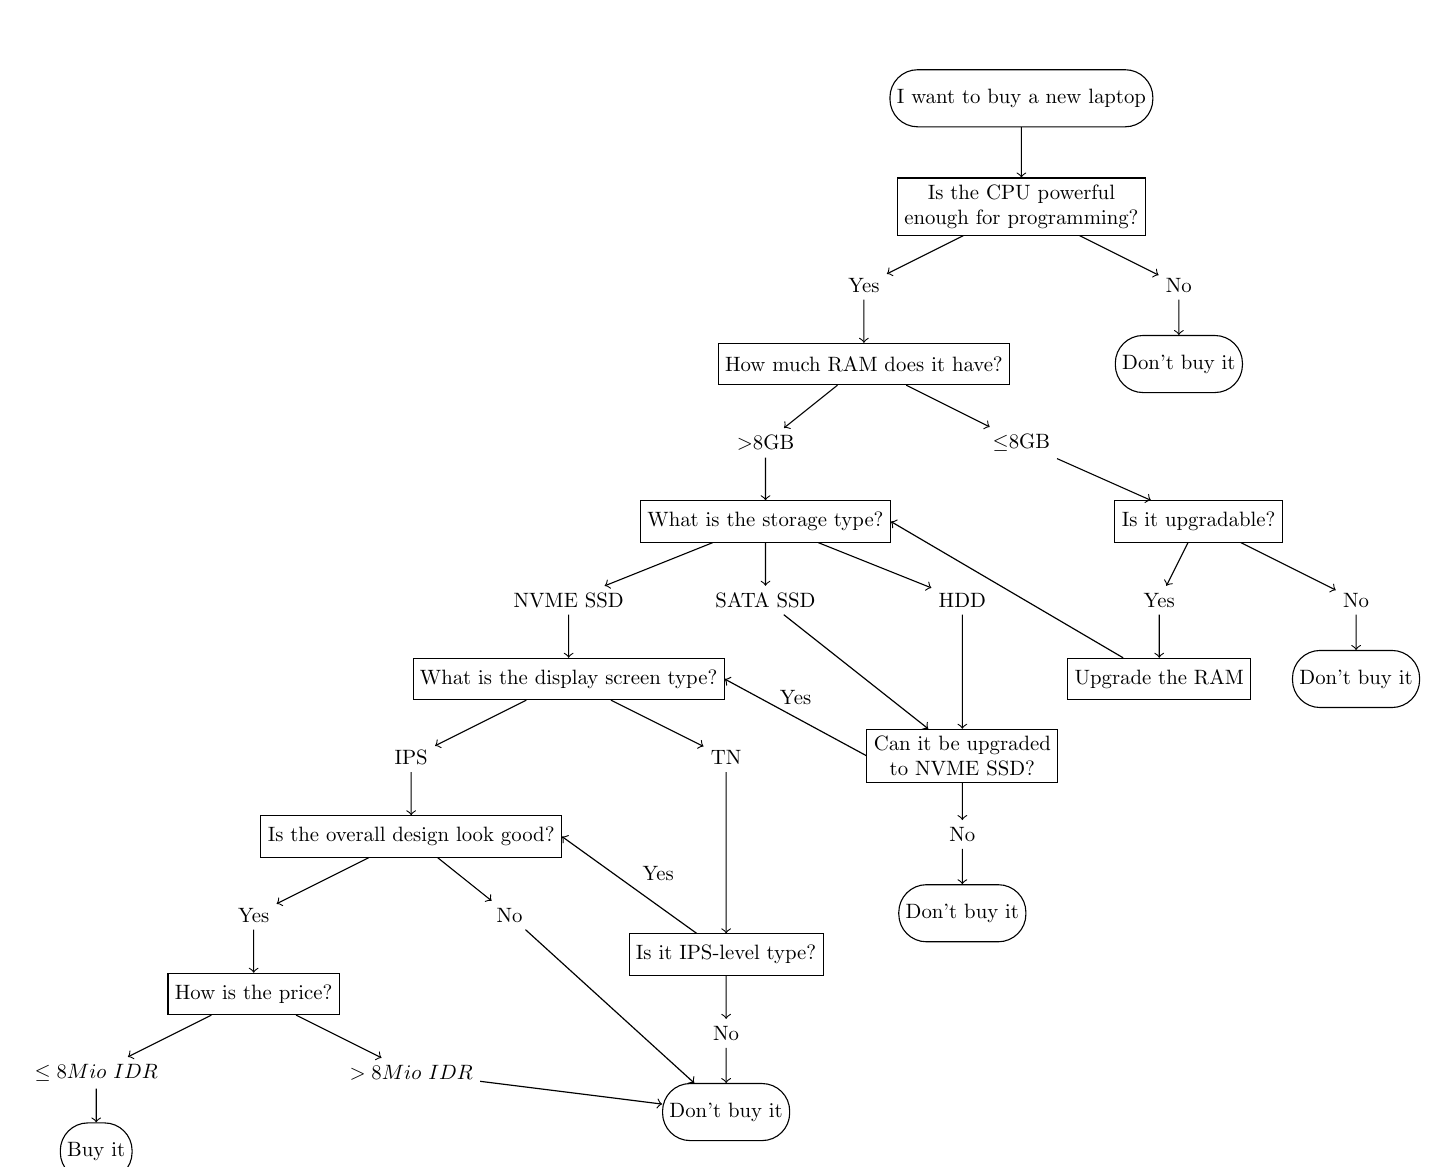
\begin{tikzpicture}[level distance=1cm,every child/.style={sibling distance=4cm},every node/.style={scale=0.75},every path/.style={->}]
        \node[terminator] {I want to buy a new laptop}
            child {node[process,align=center,yshift=-5mm] {Is the CPU powerful\\enough for programming?}
                child {node {Yes}
                    child {node[process] {How much RAM does it have?}
                        child {node[xshift=1cm] {$>$8GB}
                            child {node (storage) [process] {What is the storage type?}
                                child {node[xshift=2cm] {NVME SSD}
                                    child {node (screen-type) [process] {What is the display screen type?}
                                        child {node {IPS}
                                            child {node (design) [process] {Is the overall design look good?}
                                                child {node {Yes}
                                                    child {node[process] {How is the price?}
                                                        child {node {$\le 8Mio~IDR$}
                                                            child {node[terminator] {Buy it}}}
                                                        child {node (pricy) {$> 8Mio~IDR$}}}}
                                                child {node (bad-design) [xshift=-1cm] {No}}}}
                                        child {node {TN}
                                            child {node (ips-level) [process,yshift=-2cm] {Is it IPS-level type?}
                                                child {node {No}
                                                    child {node (tn-no-buy) [terminator] {Don't buy it}}}}}}}
                                child {node (sata-ssd) {SATA SSD}}
                                child {node[xshift=-2cm] {HDD}
                                    child {node (upgrade-storage) [process,align=center,yshift=-1.3cm] {Can it be upgraded\\to NVME SSD?}
                                        child {node {No}
                                            child {node[terminator] {Don't buy it}}}}}}}
                        child {node {$\le$8GB}
                            child {node[process,xshift=3cm] {Is it upgradable?}
                                child {node[xshift=2cm] {Yes}
                                    child {node (upgrade-ram) [process] {Upgrade the RAM}}}
                                child {node {No}
                                    child {node[terminator] {Don't buy it}}}}}}}
                child {node {No}
                    child {node[terminator] {Don't buy it}}}};
        \draw [connector] (upgrade-ram) -- (storage.east);
        \draw [connector] (sata-ssd) -- (upgrade-storage);
        \draw [connector] (ips-level) -- node[above=2mm,right=1mm] {Yes} (design.east);
        \draw [connector] (bad-design) -- (tn-no-buy);
        \draw [connector] (upgrade-storage.west) -- node[above=1mm] {Yes} (screen-type.east);
        \draw [connector] (pricy) -- (tn-no-buy);
    \end{tikzpicture}
\end{center}

\end{document}

